%% ----------------------------------------------------------------
%% SETTINGS
%% ----------------------------------------------------------------
\documentclass[../et.tex]{subfiles}

%% ----------------------------------------------------------------
%% BEGIN
%% ----------------------------------------------------------------
\begin{document}

%% ----------------------------------------------------------------
%% DOCUMENT
%% ----------------------------------------------------------------
El instrumento deberá contar con tres puertos a los cuales se puedan conectar sondas externas (sondas de Rogowski, pinzas amperométricas, etc.), para su calibración y caracterización. Uno de estos puertos será dedicado para la sonda Rogowski y los otros dos genérico para otras sondas.

El dispositivo contará con dos esquemáticos distintos para sus puertos de conexión. En la \autoref{fig:puertos-sondas} se puede observar el correspondiente para la sonda Rogowski y en la \autoref{fig:puertos-sondas-con-resistencias} el correspondiente para otras sondas.

Se incluirá además circuitos de adecuación y filtrado para cada etapa, descriptos en el esquemático de la \autoref{fig:puertos-adecuacion}.

\begin{figure}[!htbp]
  \centering
  \begin{subfigure}[b]{0.25\textwidth}
    \centering
    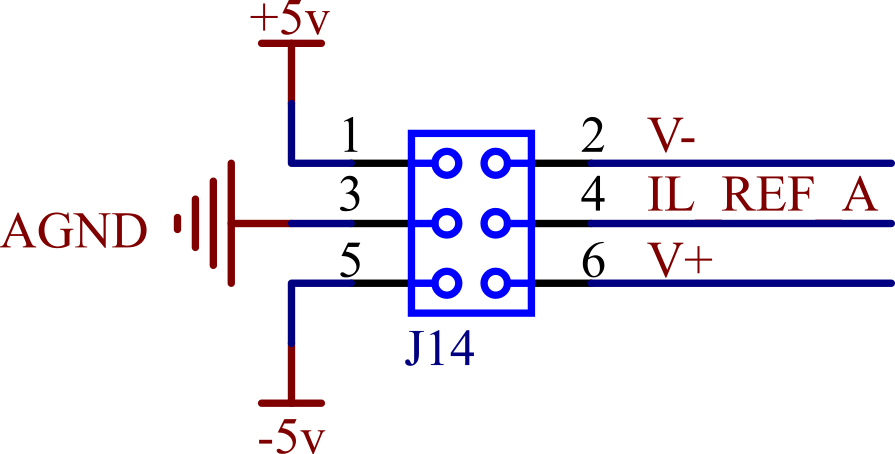
\includegraphics[width=\textwidth]{../images/puertos-sondas}
    \caption{Esquemático puerto sonda Rogowski}
    \label{fig:puertos-sondas}
    \vspace*{10mm}
  \end{subfigure}
  \hspace{0.2\textwidth}
  \begin{subfigure}[b]{0.3\textwidth}
    \centering
    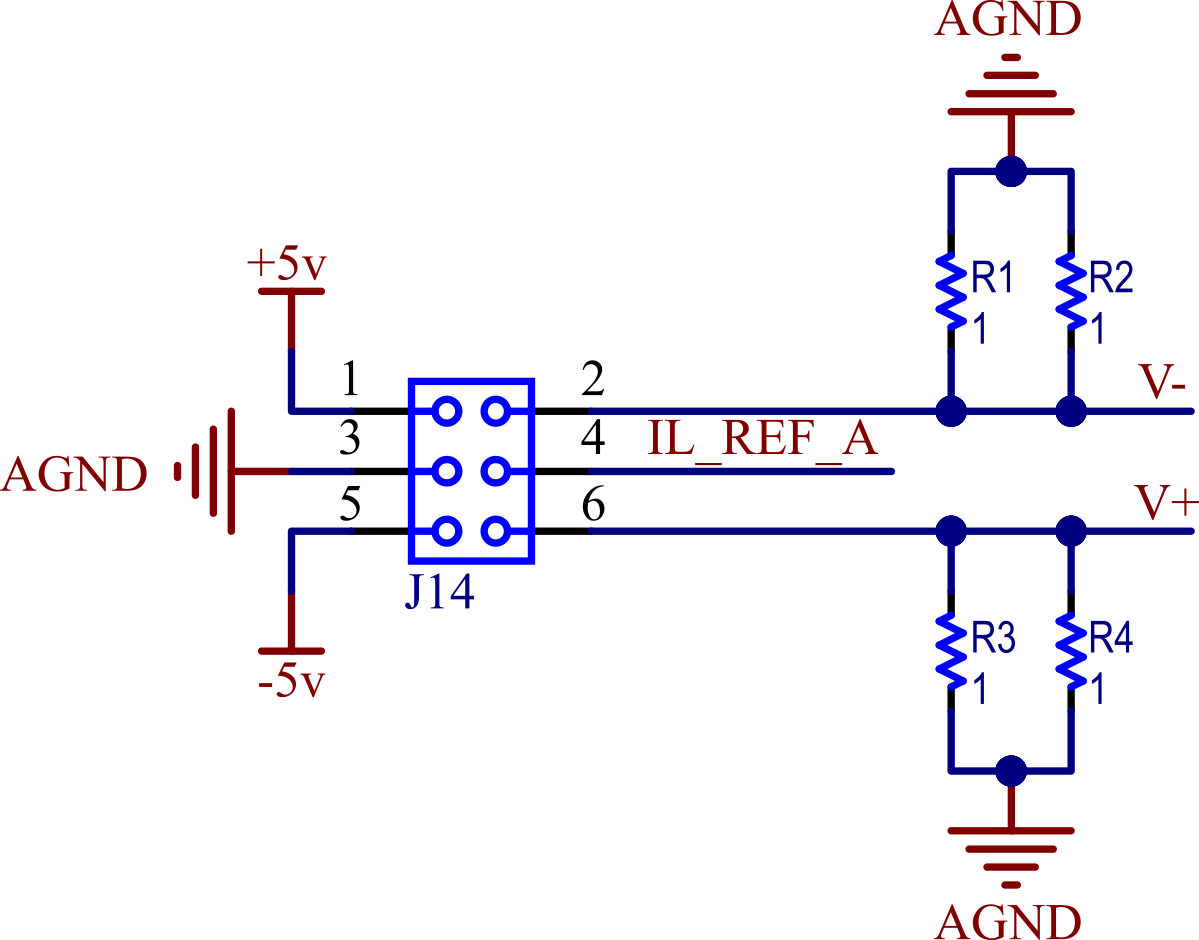
\includegraphics[width=\textwidth]{../images/puertos-sondas-con-resistencias}
    \caption{Esquemático puertos para otras sondas}
    \label{fig:puertos-sondas-con-resistencias}
    \vspace*{10mm}
  \end{subfigure}

  \begin{subfigure}[b]{0.9\textwidth}
    \centering
    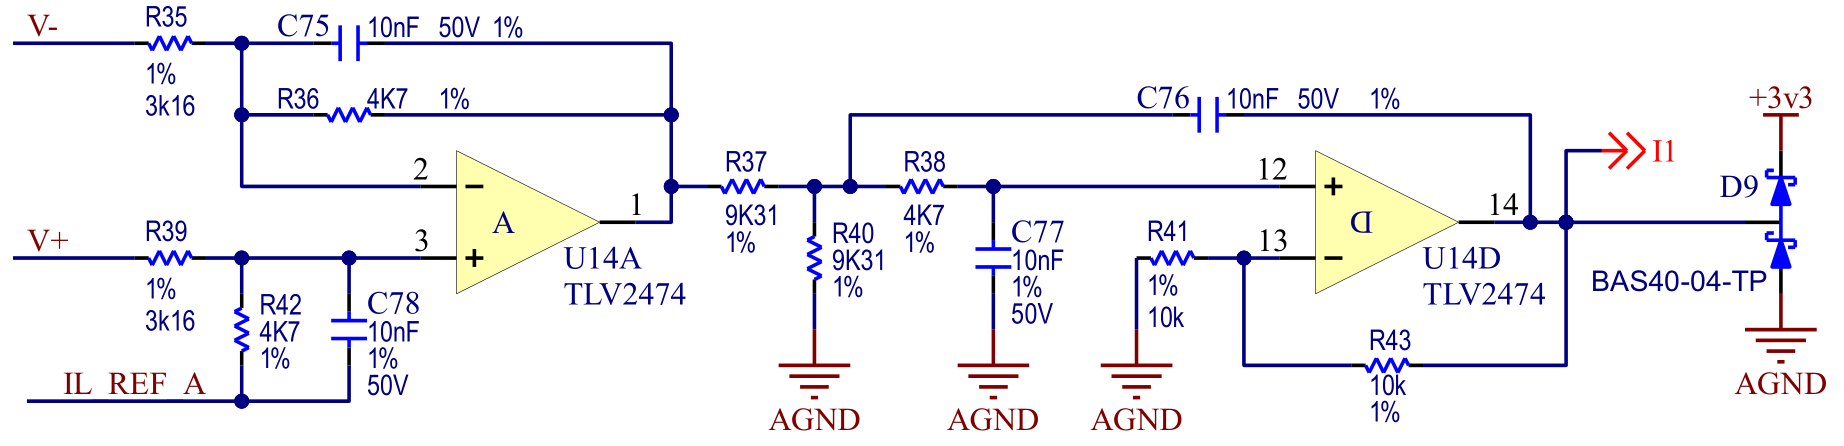
\includegraphics[width=\textwidth]{../images/puertos-adecuacion.png}
    \caption{Esquemático circuito de adecuación y filtrado}
    \label{fig:puertos-adecuacion}
    \vspace*{5mm}
  \end{subfigure}

  \label{fig:adquisicion}
  \caption{Esquemáticos etapa de adquisición}
\end{figure}

  %% ----------------------------------------------------------------
  \subsubsection{Funcionamiento}
  %% ----------------------------------------------------------------
  Este circuito proveerá la ganancia y filtrado anti-aliasing para los cuatro canales del conversor analógico digital. Los mismos, están divididos en dos tipos diferentes:
  \begin{itemize}
      \item Un canal para medir la corriente en el multiplicador. Se mide la caída de tensión de la resistencia shunt colocada en serie con la corriente que circula por la carga. Esta medición es realizada de manera de, a partir de un lazo de control, regular la corriente.
      \item Tres canales para la conexión de las sondas de corriente a caracterizar.
  \end{itemize}

  Si bien existen estos dos tipos de entradas, el circuito de adecuación y filtrado es el mismo para todas, pudiendo variar entre ellos la ganancia aplicada.

  En la \autoref{fig:adecuacion-circuito} se puede observar el circuito genérico utilizado para la adecuación y filtrado.

  \begin{figure}[!htbp]
    \centering
    \begin{circuitikz}[scale=0.6]
      \ctikzset{resistors/scale=0.6, capacitors/scale=0.6}
      % Primera etapa
      \draw (0,0)     node[op amp]    (U1) {$U_1$};
      \draw (U1.out)  to [short] ++(0.2,0) \coord(U1out);
      \draw (U1.+)    to [short, -*] ++(-1,0) \coord(U1+);
      \draw (U1+)     to [C, l=$C_2$] ++(0,-3) to [short, -o] ++(-4,0) node[left](Vref){$\frac{V_{REF}}{2}$};
      \draw (U1+)     to [short, -*] ++(-2,0) \coord(R2_b) to [R, l=$R_2$] ++(0,-3);
      \draw (R2_b)    to [R, l=$R_1$, -o] ++(-4,0) node[left](V+){$V_{in}^+$};
      \draw (U1.-)    to [short, -*] ++(-1,0) \coord(U1-);
      \draw (U1-)     to [short] ++(-2,0) to [R, l_=$R_1$, -o] ++(-4,0) node[left](V-){$V_{in}^-$};
      \draw (U1-)     to [short, -*] ++(0,2) \coord(tanque1_in);
      \draw (tanque1_in) to [C, l=$C_2$, -*] ++(5,0);
      \draw (tanque1_in) to [short] ++(0,2) to [R, l=$R_2$] ++(5,0) \coord(tanque1_out) to [short, -*] (tanque1_out |- U1out);

      % Segunda etapa
      \draw (U1out)  to [R, -*, l=$R_3$] ++(3,0) \coord(R3_out) to [R, *-, l=$R_3$] ++(0,-3) node[ground](GND){};
      \draw (R3_out) to [R, l=$R_4$, -*] ++(3,0) \coord(R4_out) to [C, l=$C_4$] ++(0,-3) node[ground](GND){};
      \draw (R4_out) to [short] ++(2,0) \coord(U2+) to [short] ++(1,0) \coord(U2);
      \draw (U2) node[op amp, anchor=+, yscale=-1] (U2) {\ctikzflipy{$U_2$}};
      \draw (U2.out) to [short, -*] ++(1,0) \coord(U2out);
      \draw (U2.-) to [short] ++(-1,0) \coord(U2-);
      \draw (U2-) to [short, -*] ++(0,-2) \coord(R5) to [R, l=$R_5$] ++(0,-3) node[ground](GND){};
      \draw (R5) to [R, l=$R_6$] ++(5,0) \coord(R5out) to [short] (R5out |- U2out);
      \draw (R3_out) to [short] ++(0,2) to [C, l=$C_4$] ++(10,0) \coord(C4out) to [short, -*] (C4out |- U2out);
      \draw (U2out) to [short, -o] ++(0,0) node[right](Vout){$V_{out}$};
    \end{circuitikz}
    \caption{Circuito de adecuación y filtrado}
    \label{fig:adecuacion-circuito}
  \end{figure}

  %% ----------------------------------------------------------------
  \paragraph{Primera etapa}
  %% ----------------------------------------------------------------
  En esta etapa que culmina en la salida del primer amplificador operacional $U_1$, se incluye una configuración diferencial junto con un filtro pasabajos de primer orden. La transferencia de esta etapa es la siguiente:
  \[
    \frac{V_1(s)}{V_{in}^+(s) - V_{in}^-(s)} = \frac{R_2}{R_{1} } \cdot \frac{1}{1+sC_{2}R_{2}}
  \]

  %% TODO: justificar 3400 Hz
  De manera de tener una frecuencia de corte de aproximadamente \SI{3400}{Hz}, se eligieron los siguientes valores:
  \begin{itemize}
    \item $R_2 = \SI{4.7}{k \ohm}$
    \item $C_2 = \SI{10}{nF}$
  \end{itemize}

  Se obtuvo de esta forma una frecuencia de corte $f_c = \SI{3386}{Hz}$. La resistencia $R_1$ se elegirá de acuerdo a las necesidades de ganancia de cada entrada.

  Los amplificadores operacionales son alimentados en forma unipolar, por lo que se emplea una tensión de offset de $\frac{V_{REF}}{2}$.

  %% ----------------------------------------------------------------
  \paragraph{Segunda etapa}
  %% ----------------------------------------------------------------
  Filtro pasabajos de segundo orden tipo Sallen-Key.

  Si se observa la \autoref{fig:adecuacion-circuito-sallenkey}, se verá una de las configuraciones más comunes encontradas en la literatura \cite{ti:sloa024b}.

  \begin{figure}[!htbp]
    \centering
    \begin{circuitikz}[scale=0.6]
      \ctikzset{resistors/scale=0.6, capacitors/scale=0.6}
      % Segunda etapa
      \draw (0,0) node[left](Vin){$V_i$} to [R, l=$R_3$, o-] ++(4,0) \coord(R3_out);
      \draw (R3_out) to [R, l=$R_4$, *-] ++(3,0) \coord(R4_out) to [C, l=$C_3$, *-] ++(0,-3) node[ground](GND){};
      \draw (R4_out) to [short] ++(2,0) \coord(U2+) to [short] ++(1,0) \coord(U2);
      \draw (U2) node[op amp, anchor=+, yscale=-1] (U2) {\ctikzflipy{$U_2$}};
      \draw (U2.out) to [short] ++(1,0) \coord(U2out);
      \draw (U2.-) to [short] ++(-1,0) \coord(U2-);
      \draw (U2-) to [short, -*] ++(0,-2) \coord(R5) to [R, l=$R_5$] ++(0,-3) node[ground](GND){};
      \draw (R5) to [R, l=$R_6$] ++(5,0) \coord(R5out) to [short, -*] (R5out |- U2out);
      \draw (R3_out) to [short] ++(0,2) to [C, l=$C_4$] ++(10,0) \coord(C4out) to [short] (C4out |- U2out);
      \draw (U2out) to [short, -o] ++(0,0) node[right](Vout){$V_{o}$};
    \end{circuitikz}
    \caption{Configuración Sallen-Key pasabajos estándar}
    \label{fig:adecuacion-circuito-sallenkey}
  \end{figure}

  La transferencia de un circuito Sallen-Key en la configuración de la \autoref{fig:adecuacion-circuito-sallenkey} es la siguiente:
  \[
    \frac{V_o(s)}{V_i(s)} = \frac{K}{s^2(R_3R_4C_3C_4) + s(R_3C_3+R_4C_3+R_3C_4(1-K)) + 1}
  \]
  siendo:
  \[
    f_c = \frac{1}{2\pi \sqrt{R_3R_4C_3C_4}} \qquad \text{y} \qquad Q = \frac{\sqrt{R_3R_4C_3C_4}}{R_3C_3+R_4C_3+R_3C_4(1-K)}
  \]

  Para acelerar el diseño, se pueden encontrar en la literatura diversas simplificaciones \cite{ti:sloa024b}. En este caso, se ha decidido optar por igualar componentes. Así, $R_3 = R_4 = R$ y $C_3 = C_4 = C$, resultando en:
  \[
    f_c = \frac{1}{2\pi RC} \qquad \text{y} \qquad Q = \frac{1}{3 - K}
  \]

  Así, se eligió utilizar un factor $Q=1$ que, utilizando resistencias con margen de error de $1 \%$, resultaría para un peor caso un factor $Q=1.02$.

  Habiendo realizado esta elección, y siendo este el único grado de libertad del circuito, se obtiene $K=2$. Es por ello que, tal como se mencionó antes, se realiza la modificación en la resistencia $R_3$. Al atenuar la señal a la mitad con el divisor resistivo antes de introducirla a la segunda etapa, se cancela el efecto de ganancia de esta última, quedando así, a fines prácticos, una ganancia unitaria. La única condición necesaria es ahora:
  \[
      \frac{R_3}{2} = R_4
  \]
  de manera de cumplir la simplificación planteada.

  Atendiendo a todas estas consideraciones y cumpliendo la frecuencia de corte antes planteada, se eligieron los siguientes valores:
  \begin{itemize}
      \item $R_3 = \SI{9.31}{k\ohm}$
      \item $R_4 = \SI{4.7}{k\ohm}$
      \item $C_3 = C_4 = \SI{10}{nF}$
      \item $R_5 = R_6 = \SI{10}{k\ohm}$
  \end{itemize}
  utilizando de esta manera los mismos componentes que en la etapa previa, llegando a la frecuencia de corte de \SI{3386}{Hz}, logrando el filtro pasabajos de tercer orden deseado.

  %% ----------------------------------------------------------------
  \subsubsection{Protección ADC}
  %% ----------------------------------------------------------------
  En el circuito final, se agregaron dos diodos schottky a la salida, uno conectado a \SI{3.3}{V} y el otro a masa para la protección de las entradas del conversor analógico digital, limitando la tensión máxima a $\SI{3.3}{V} + V_F$, siendo $V_{F_{max}} = \SI{1}{V}$ para el integrado elegido.

  %% ----------------------------------------------------------------
  \subsubsection{Puertos de conexión}
  %% ----------------------------------------------------------------
  Para los puertos de conexión, se incluirá en ambos casos salidas de \SI{\pm 5}{V}, junto con una salida de masa, para conectar las sondas que las requieran. Se agregará también una salida con la tensión de referencia utilizada en la etapa de adecuación.

  En el caso del puerto genérico se agregará una serie de resistencias que permita generar una tensión medible a partir de la corriente de entrada. Las mismas no serán montadas en la construcción y se dejará al usuario decidir los valores de acuerdo a la necesidad de la sonda que desee conectar.

  Los puertos físicos podrán ser elegidos por el desarrollador.

\end{document}